\documentclass[10pt]{beamer}
\usepackage{lmodern}
\usepackage{amssymb}
\usepackage{graphicx}
\usepackage{amsmath}
\usepackage{multirow}
\usepackage{mathtools}
\usepackage{placeins}
\usepackage{lscape}
\usepackage{geometry}
\usepackage{dcolumn}
\usepackage[utf8]{inputenc}
\usepackage{hyperref}
\usepackage{tabularx}
\usepackage{nicematrix}
\usepackage{calc}
\usepackage{qtree}
\usepackage{tikz}
\usetikzlibrary{shapes.geometric, arrows}

\usetheme{Boadilla}


\title{SOFR so good? New Benchmark Rate and Crowding-Out Effect}  
\author{Qian Wu}
\date{\today} 

\makeatletter
\newcommand\MyInfo[1]{%
\setbeamertemplate{footline}
{
  \leavevmode%
  \hbox{%
  \begin{beamercolorbox}[wd=.22\paperwidth,ht=2.25ex,dp=1ex,center]{author in head/foot}%
    \usebeamerfont{author in head/foot}#1
  \end{beamercolorbox}%
  \begin{beamercolorbox}[wd=.56\paperwidth,ht=2.25ex,dp=1ex,center]{title in head/foot}%
    \usebeamerfont{title in head/foot}\insertshorttitle
      \end{beamercolorbox}%
  \begin{beamercolorbox}[wd=.22\paperwidth,ht=2.25ex,dp=1ex,right]{date in head/foot}%
    \usebeamerfont{date in head/foot}\insertshortdate{}\hspace*{2em}
    \insertframenumber{} / \inserttotalframenumber\hspace*{2ex} 
  \end{beamercolorbox}}%
  \vskip0pt%
}
}
\makeatother

\tikzstyle{io} = [rectangle, rounded corners, minimum width=3cm, minimum height=.7cm,text centered, draw=black, fill=blue!30]
\tikzstyle{arrow} = [thick,->,>=stealth]


\begin{document}
\MyInfo{Qian Wu}


\begin{frame}
\titlepage
\end{frame} 


\begin{frame}
\frametitle{Background Info}
\begin{itemize}
\item LIBOR has been the reference interest rate used worldwide in a large variety of financial assets including business loans,  consumer loans,  and derivatives.
\item Due to the LIBOR manipulation scandal and a shrinking interbank debt market,  LIBOR is being retired \footnote{The publication for one-week and two-month USD LIBOR will cease on December 31, 2021; the publication for the USD LIBOR with other terms will cease on June 30, 2023.}.  In the US,  the Alternative Reference Rate Committee (ARRC) recommends SOFR as the alternative to the USD LIBOR.
\item \textbf{LIBOR}: London Interbank Offered Rate
\begin{itemize}
\item LIBOR is the average interest rate that leading banks borrow from each other. 
\item  It's based on banks' own estimation,  not real transactions.
\end{itemize}
\item \textbf{SOFR}: Secured Overnight Financing Rate
\begin{itemize}
\item SOFR is a broad measure of the cost of borrowing cash overnight collateralized by Treasury securities.
\item It's based on the real transactions in the overnight Treasury repurchase market.
\end{itemize}
\end{itemize}
\end{frame}



\begin{frame}
\frametitle{Research Question}
Does the change of the benchmark interest rate affect the size of the government debt crowding out effect?
\begin{itemize}
\item \textbf{Crowding-Out Effect}: Gov't issues more Treasuries $\rightarrow$ Demand for loanable funds increases $\rightarrow$ Interest rate increases $\rightarrow$ Private spending decreases
\item Since SOFR is based on transactions collateralized by Treasuries,  the economy with SOFR may obtain a different magnitude of crowding-out effect.
\end{itemize}
\end{frame}


\begin{frame}
\frametitle{Scarce Collateral Channel}
\begin{itemize}
\item In economy with SOFR,  the crowding-out effect can be amplified through the following channel:
\begin{itemize}
\item Gov't issues Treasuries $\xrightarrow {\text{}}$ Scarce collateral effect causes a higher demand for borrowings collateralized with Treasuries $\xrightarrow {\text{}}$ SOFR rises $\xrightarrow {\text{}}$ Business loans become more costly $\xrightarrow{\text{}}$ Investment decreases
\end{itemize}
\end{itemize}
\end{frame}



\begin{frame}
  \frametitle{\large Business Loans in Total Debt for Nonfinancial Sectors}
  \begin{center}
  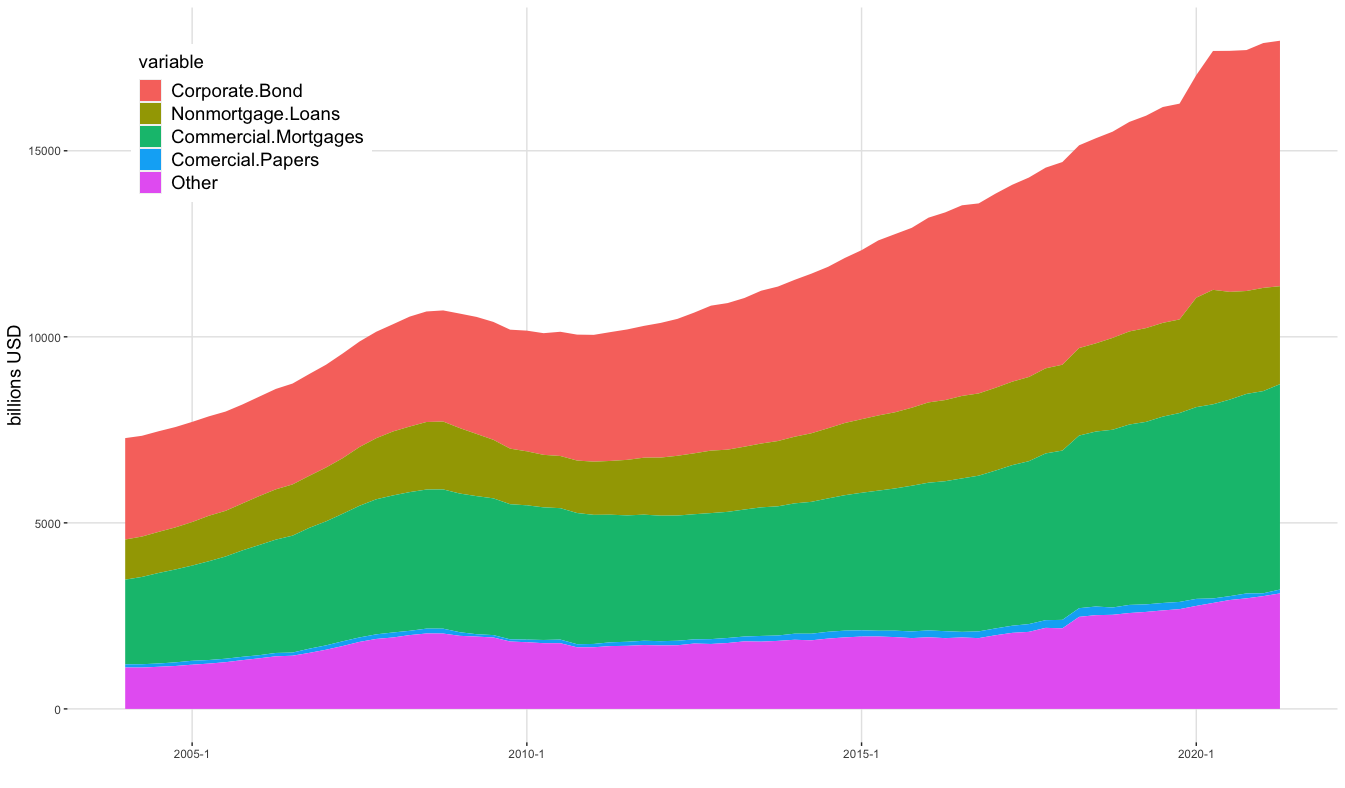
\includegraphics[scale=.22]{businessdebt.png}\\
  \tiny Fig 2: Components of National Business Debts
  \end{center}
\end{frame}



\begin{frame}
  \frametitle{Business Loans Indexed by LIBOR}
  A considerable scale of business loans were indexed by LIBOR.
  \begin{center}
  {\footnotesize%
  \begin{tabular}{lc}
  \multicolumn{2}{c}{Table 1: Estimated Business Loans Exposed to USD LIBOR}\\\hline
   &Volume \\ 
   &(Trillions USD)  \\ \hline
   Syndicated loans & 1.5 \\
   Nonsyndicated loans & 0.8  \\
   Commercial mortgages & 1.1  \\
   \hline \hline
  \multicolumn{2}{l}{ Source: Second Report of The Alternative Reference Rates Committee.} \\
  \multicolumn{2}{l}{Note: Data are gross national exposures as of year-end 2016.  }\\
  \multicolumn{2}{l}{\hspace{7mm} At of year-end 2016,  total national nonfinancial business nonmortgage loan is 4.1} \\ 
  \multicolumn{2}{l}{\hspace{7mm} trillions of USD and total commercial mortgage is 4.2 trillions of USD. }
  \end{tabular}
  }%
  \end{center}
  \end{frame}
  

  
  \begin{frame}
  \frametitle{Banks Picking up SOFR}
  Leading banks have explicitly or implicitly indicated that they will pick up SOFR as the replacement for LIBOR.
  \begin{itemize}
  \item \textbf{JPMorgan Chase}: All new loan financings, such as for mergers and acquisitions that JPMorgan is underwriting are being tied to SOFR if they are expected to price next year, said Kevin Foley, the bank's global head of capital markets. (Financial Times)
  \item \textbf{BOA}: Grabenstein added Wells Fargo has not "put a total stop on LIBOR loans, but we are going to the customer with SOFR first and only if there is a real need to use LIBOR should it still be considered." (Financial Times)
  \item \textbf{U.S.  Bank}: U.S. Bank became operationally ready to offer SOFR for most commercial loans.  (U.S.Bank website)
  \item \textbf{Truist}: At Truist we offer SOFR as an alternative rate for commercial loans...(Truist website)
  \item \textbf{TD Bank}: For LIBOR indexed loans with tenors after the anticipated phase-out date, we plan to offer three SOFR varieties based on customer preference or appropriateness as alternatives to LIBOR after the phase-out date.  (TD Bank website)
  \end{itemize}
  \end{frame}
  



\begin{frame}
\frametitle{OLS: SOFR and Gov't Debt}
\begin{itemize}
\item Regress SOFR and LIBOR spread over FFR on government debt outstanding.
\begin{center}
  {\scriptsize%
\begin{tabular}{@{\extracolsep{1pt}}lD{.}{.}{-3} D{.}{.}{-3} D{.}{.}{-3} D{.}{.}{-3} } 
\multicolumn{5}{c}{Table 3: Response of SOFR and LIBOR to Government Debt Issuance}\\[.8ex]\hline 
\hline \\[-1.8ex] 
 & \multicolumn{4}{c}{\textit{Dependent variable:}} \\ 
\cline{2-5} 
\\[-1.8ex] & \multicolumn{2}{c}{SOFR spread} & \multicolumn{2}{c}{LIBOR spread} \\ 
\\[-1.8ex] & \multicolumn{1}{c}{(1)} & \multicolumn{1}{c}{(2)} & \multicolumn{1}{c}{(3)} & \multicolumn{1}{c}{(4)}\\ 
\hline \\[-1.8ex] 
Government debt & 614.474^{***} & 609.553^{***} & -36.676 & -34.162 \\ 
  & (166.458) & (169.146) & (23.319) & (22.558) \\ 
  Lagged SOFR &  & 0.173^{**} &  &  \\ 
  &  & (0.078) &  &  \\ 
  Lagged LIBOR &  &  &  & -0.163^{**} \\ 
  &  &  &  & (0.066) \\ 
  Constant & -0.276^{***} & -0.242^{***} & 0.008 & 0.008 \\ 
  & (0.088) & (0.068) & (0.010) & (0.011) \\ 
 \hline \\[-1.8ex] 
Adjusted $R^2$ & 0.0405 & 0.0696 & 0.0026 & 0.0283 \\ 
Observations & 1135 & 1134 & 1100 & 1082 \\ 
 \hline \\[-1.8ex] 
\hline 
 \multicolumn{5}{l}{Note: $^{*}$p$<$0.1; $^{**}$p$<$0.05; $^{***}$p$<$0.01} \\ 
 \multicolumn{5}{l}{\hspace{7mm}All variables are in diff log format.}\\
\multicolumn{5}{l}{\hspace{7mm}Newey-West Standard Error in parenthesis.}\\
\multicolumn{5}{l}{\hspace{7mm}The sample includes daily data from August 25, 2014 to December 31, 2019.}
\end{tabular} 
}%
\end{center}
\item The results show that issuing government debt is correlated with higher SOFR level while it has no significant effect on LIBOR.
\end{itemize}
\end{frame}




\begin{frame}
  \frametitle{LP: Effect of Gov't Borrowing Shock}
Two Steps:
\begin{itemize}
  \item Compute government borrowing shocks
  \begin{align*}
    b_t=\alpha_0+\alpha_1t+\alpha_2t^2+A(L)X_{t-1}+\epsilon_t^b
  \end{align*}
  \begin{itemize}
    \item $b_t$: log(govt debt)
    \item $X_t$: controls including six lags of log(govt debt), log(industrial production), and log(stock price)
    \item $\hat{\epsilon}_t^b$: identified borrowing shock
  \end{itemize}
  \item Estimate local projections
  \begin{align*}
    r_{t+h}=\beta_0+\psi_h \hat{\epsilon}_t^b +\Gamma(L)Z_{t-1}+u_{t+h}
  \end{align*}
    \begin{itemize}
      \item $r_{t+h}$: SOFR or LIBOR spread at horizon h
      \item $Z_{t-1}$: controls including three lags of SOFR or LIBOR spread, log(govt debt), and log(industrial production)
    \end{itemize}
\end{itemize}
\end{frame}


\begin{frame}
  \frametitle{LP: Results}
  \begin{center}
    IRFs of Government Borrowing Shock
    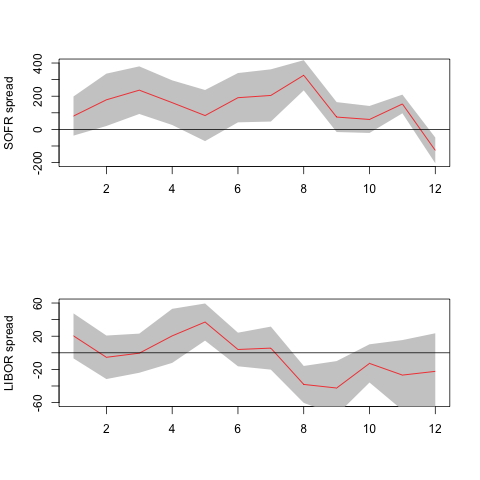
\includegraphics[scale=0.5]{irfs.png}
  \end{center}
\end{frame}


\begin{frame}
  \frametitle{Model}
  \begin{itemize}
    \item An RBC model with financial frictions based on Walque, Pierrard, and Rouabah (2010). 
    \item The direct borrowing between firms and households is not feasible, funds must flow through an interbank lending market.
    \item Deposit banks demand deposits from households, they lend to commercial banks through the interbank lending market.
    \item In economy under SOFR, commercial banks borrow from deposit banks through the interbank market using government bonds as collateral.
    \item Firms borrow uninsuredly from the merchant banks for business capital.
    \item Commercial banks and firms are allowed to default, while deposit banks cannot default.
  \end{itemize}
\end{frame}



\begin{frame}
  \frametitle{Households}
  \begin{itemize}
    \item Households choose consumption $C_t$ and deposits $D_t$ to maximize their expected lifetime utility subject to flow budget constraint.
    \item They receive labor income $w_tN$ and pay lump-sum tax $T_t$.
    \item They own deposit banks, commercial banks, and firms.
  \end{itemize}
  \begin{align}
    &\max_{\{c_t, D_t\}} E \sum_{t=0}^{\infty} \beta^t logC_t ,\\
    s.t. \nonumber \\
    &C_t+\frac{D_t}{1+r_t}+T_t=w_tN+D_{t-1}+d_t^D+d_t^C+d_t^F
  \end{align}
\end{frame}



\begin{frame}
\frametitle{Deposit Banks}
  \begin{itemize}
    \item Deposit banks choose deposit demand $D_t$ and interbank lending supply $I_t$ to maximize profits.
    \item Interbank lending requires collateral in the form of government bonds $B_t$. For the part of lendings on which the merchant banks choose to default ($1-\gamma_t^I$), the deposit banks will recover
    a fraction $\theta$ of the collateralized assets. 
  \end{itemize}
  \begin{align}
    &\max_{\{D_t, I_t, d_t^D\}} E \sum_{t=0}^{\infty} \{M_t d_t^D\} ,\\
    s.t. \nonumber \\
    &d_t^D=\gamma_t^I I_{t-1}+\frac{D_t}{1+r_t}-D_{t-1}-\frac{I_t}{1+r_t^I}+ \theta(1-\gamma_{t-1}^I)I_{t-2},\\
  \end{align}
\end{frame}



\begin{frame}
  \frametitle{Commercial Banks}
\begin{itemize}
  \item Commercial banks choose interbank lending demands $I_t$, government bonds holding $B_t$, business loan supply $L_t$, and repayment rate $\gamma_t^I$ to maximize its profits. 
  \item Interbank borrowing features a collateral requirement. There is no haircut for government bonds as a collateral.To simplify the problem, it's assumed that commercial banks borrow at their limit.
  \item Two types of default costs: (1) a fraction $\theta$ of collateral is forfeited; (2) non-pecuniary cost $\xi_C(1-\gamma_t^I)$.
\end{itemize}
\begin{align}
  &\max_{\{I_t, B_t, L_t, \gamma_t^I, d_t^C\}} E \sum_{t=0}^{\infty} \{M_t d_t^C\} ,\\
  s.t. \nonumber \\
  &d_t^C=\gamma_t^L L_{t-1}+\frac{I_t}{1+r_t^I}-\gamma_t^I I_{t-1}-\frac{L_t}{1+r_t^L} \nonumber \\
  & \hspace{3cm}-\theta(1-\gamma_{t-1}^I)I_{t-2}-\xi_C(1-\gamma_t^I)+B_{t-1}-\frac{B_t}{1+r_t^B}, \\
  &I_t= B_t 
\end{align}
\end{frame}


\begin{frame}
  \frametitle{Firms}
  \begin{itemize}
    \item Firms choose labor demand $N_t$, business loan demand $L_t$, and repayment rate $\gamma_t^L$ to maximize profits. 
    \item They can default on business loans with a non-pecuniary cost $\xi_F(1-\gamma_t^L)$.
  \end{itemize}
  \begin{align}
    &\max_{\{N_t, L_t, \gamma_t^L, d_t^F, K_t\}} E \sum_{t=0}^{\infty} \{ M_t d_t^F \} ,\\
    s.t. \nonumber \\
    &K_t=(1-\delta)K_{t-1}+\frac{L_t}{1+r_t^L}, \\
    &d_t^F=F(K_t, N_t)-w_tN_t-\gamma_t^L L_{t-1}-\xi_F(1-\gamma_t^L)
  \end{align}
\end{frame}

\begin{frame}
  \frametitle{Gov't Budegt Constraint}
  \begin{align}
    G_t+B_{t-1}=\frac{B_t}{1+r_t^B}+T_t
  \end{align}
\end{frame}



\end{document}

